% !TEX root = ../TAMU_Thesis_Main.tex
%%%%%%%%%%%%%%%%%%%%%%%%%%%%%%%%%%%%%%%%%%%%%%%%%%%
%
%  New template code for TAMU Theses and Dissertations starting Fall 2016.
%
%  Author: Sean Zachary Roberson 
%	 Version 3.08.16
%  Last updated 8/19/2016
%
%  Modified 04 Nov. 2016 by Kyle R. Wodzicki
%%%%%%%%%%%%%%%%%%%%%%%%%%%%%%%%%%%%%%%%%%%%%%%%%%%

%%%%%%%%%%%%%%%%%%%%%%%%%%%%%%%%%%%%%%%%%%%%%%%%%%%%%%%%%%%%%%%%%%%%%%
%%                           SECTION I
%%%%%%%%%%%%%%%%%%%%%%%%%%%%%%%%%%%%%%%%%%%%%%%%%%%%%%%%%%%%%%%%%%%%%

\chapter{Introduction and Literature Review}

\section{Author's Message to the Student Using This Template For Their Thesis or Dissertation}

Howdy! This is the template for theses and dissertations written using \LaTeX for submission at Texas A\&M University. The Office of Graduate and Professional Studies (OGAPS) is here to guide you in submitting your thesis or dissertation. This template shows the many features of \LaTeX, with many more available to the user.

There are numerous guides, references, and tutorials available on the Internet to help you. If you are stuck, don't be afraid to conduct a Google search for your issue, or you can contact me at szroberson@exchange.tamu.edu or ogaps-latex@tamu.edu.


\subsection{Brief Usage of the Template}

This template is intended for use by STEM\footnote{Science, Technology, Engineering, and Mathematics. This is an example of a footnote. You can see that it is numbered and appended at the end of the page. Also, you can see the effect of having a multiline footnote.} students. If you are not a STEM student, this template is likely not for you.

The advantage of using this template over the Microsoft Word templates are numerous. First, there is a lot of control granted to the user in how the document looks. Of course, you are expected to still follow the guidelines set forth in the TAMU Thesis Manual. This template takes care of the margins, heading requirements, and front matter ordering for you.


\subsection*{Software to Install}

\textbf{MikTeX} or \textbf{ProTeXt} is the free software recommended for Windows PC users to
compile your \LaTeX ~ document. To compile for this document, XeLaTeX compiling engine
is used. There is currently an issue in which the package xetex-def does not install; see the file README.txt for a solution. Another software called \textbf{JabRef} is also recommended for bibliography/reference management; its usage is similar with EndNote.

\subsection*{Procedure to Compile \LaTeX ~ Document}

This template (and consequently, your document) will be compiled using XeLaTeX. To compile your document, do the following\footnote{Notice here that I also show off the itemize environment for unordered lists. Ordered lists use the enumerate environment.}:

\begin{itemize}
	\item In TeXstudio, go to the Tools menu, then select Commands, and click XeLaTeX.
	
	\item In Texmaker, go to the Tools menu and select XeLaTeX.
	
	\item For other editors, consult the help files included with the editor.
\end{itemize}

To view the output after the program is done compiling, press F7 in TeXstudio and TeXmaker or the appropriate hotkey for other editors. Be sure that the document is not open in another PDF reader, for your editor will not display it.

\subsection{How to Fill This Document}
The document structure is organized in the main .tex file, TAMUTemplate.tex,
which has the same name as the output PDF file. Content in each section is in the data folder. You can open the .tex files under the data folder to modify. Four sections
are added initially. To add in more sections into the \LaTeX document, open the
TAMUTemplate.tex file and go to \textbf{line 130} you can just delete the content in the data folder and fill your documents and then compile under TAMUTemplate.tex.)

\subsection{Reference Usage and Example}

This subsection tests the usage of references. The book\cite{REALCAR} 
is referred in this way. Actually, the option is available for you to change the default way how reference appears. The default and most commonly used option \cite{einstein} is displayed here \cite{Barn-JORVQ}.

Unrelated citations are referred here for the test of reference section only\cite{TAMU}. If you
find that the reference \cite{GIGEM} has more items than you need \cite{WAGFJ}, question marks will show up in place of a reference handle, like these \cite{Over9000}.

\subsection{Equations, Formulas, and Other Really Cool Math Things That \LaTeX ~ Can Do}

Equations can be written in \LaTeX ~ in one of two ways. First, you can have material displayed inline by enclosing the desired statement in dollar signs. For example, $e^{i\pi}+1=0$ is an inline math expression. Some longer expressions, especially those including sums, integrals, or large operators and objects can be displayed centered on their own line. In this \textbf{math mode}, you enclose the desired material in square brackets. For example,

\[ \sum_{j = 1} ^n \int f_j \ dx = \int \sum_{j = 1} ^n f_j \ dx \]
is a math mode expression. We can also have a series of expressions aligned at a symbol. This is particularly useful when you are showing details in solving an equation or evaluating an integral. The next block shows off the \textit{align*} environment. We use it here to show a distributive property of set intersections over unions. Observe how each line is aligned to the biconditional symbol. This makes reading steps easier, since a reader can go line by line and determine why each step is justified.

\begin{align*}
x \in A \cap \bigcup_{j} B_j &\iff x \in A \ \wedge \ x \in \bigcup_{j} B_j \\
&\iff x \in A \ \wedge \ x \in B_k \ \text{ for some k} \\
&\iff x \in \bigcup_{j} A \cap B_j
\end{align*}

There are many more commands and features available, but this document is too small to contain them.\footnote{Yes, I pulled a Fermat. But really, a Google search will likely help you find what you need to do.} Many guides are available on the Internet for your use.

%Have some material about the align environments. Include also the eqn environment.

\subsection{A Test Section}

This is just a test. Below is a figure displaying some Haskell code in a compiler.

\begin{figure}[!ht]
\centering
	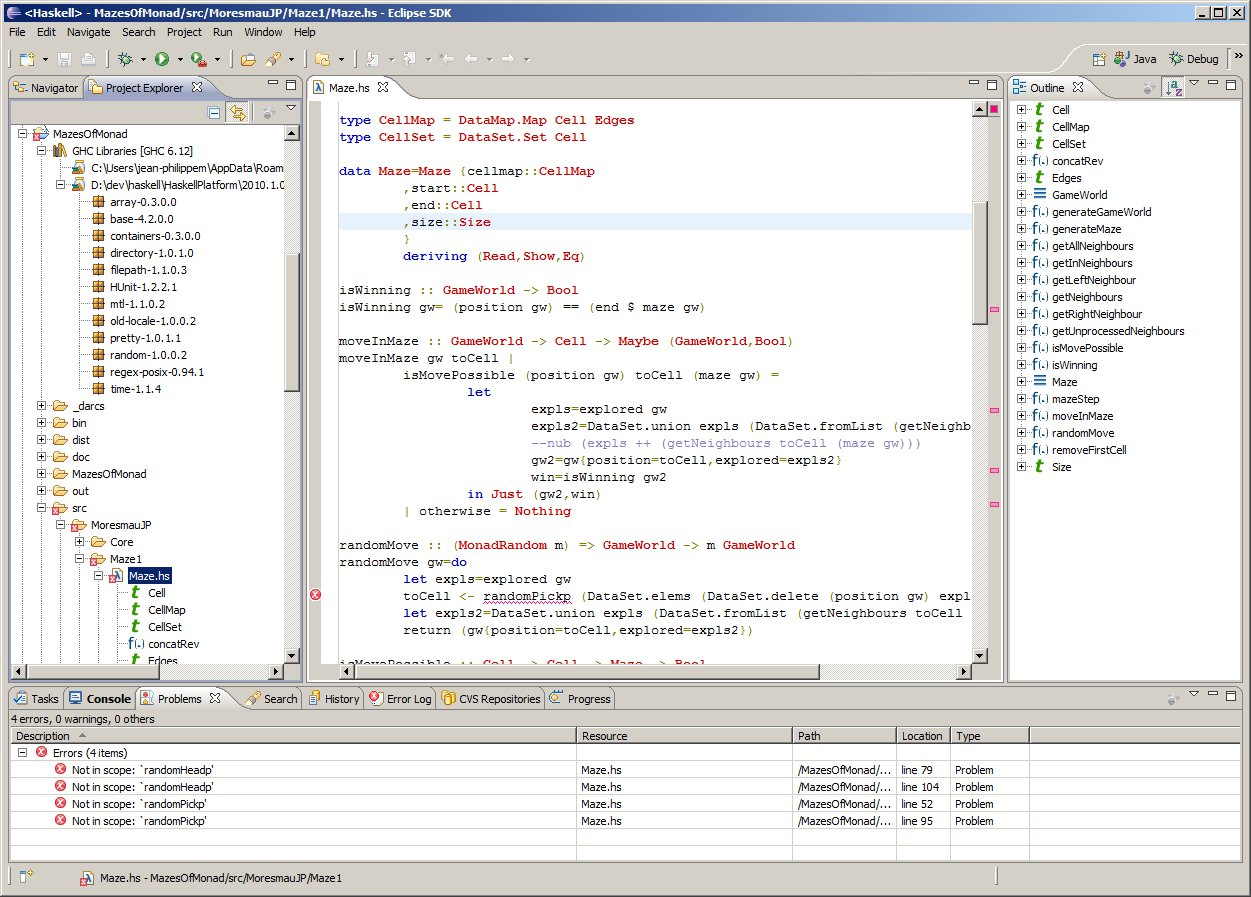
\includegraphics[scale=0.26]{Haskell1.jpg}
	\caption{Some Haskell code in a compiler.}
\end{figure}

This template has been designed for use in modern systems, but can perhaps be adapted to work on older systems, such as Windows 95. Below is a screenshot of a DOSBox console, an MS-DOS emulator designed to work on several platforms. Windows 95 can be installed into DOSBox, but it is not suggested.

\begin{figure}[ht!]
\centering
	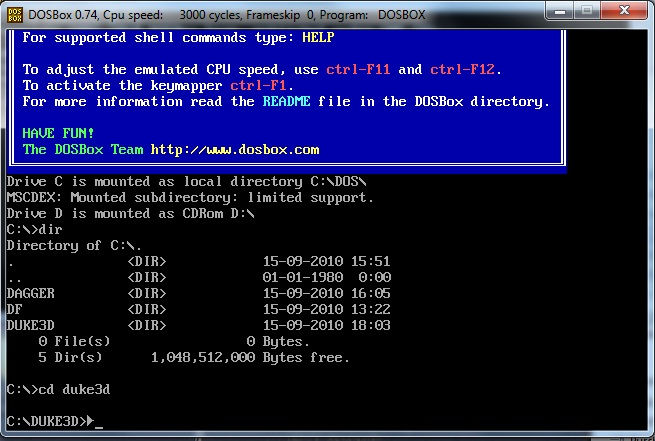
\includegraphics[scale=0.85]{DOSBox1.jpg}
	\caption{The DOSBox console running in Windows 7. The contents of the mounted directory C: are displayed, with the active subdirectory DUKE3D.}
\end{figure}

\section{Specifications in This TAMU \LaTeX ~ Template}

All requirements for theses can be found in the most recent version of the Thesis Manual, available at the OGAPS website. The Thesis Office will be happy to assist you if you have questions about formatting. Questions specific to \LaTeX\ should be directed to \texttt{ogaps-latex@tamu.edu}.

A common question students ask is the placement of a copyright statement at the beginning of a section with reprinted material from a previously printed source. The screenshot below describes how to achieve this. Check the instruction files for more details.

\begin{figure}[ht!]
\centering
	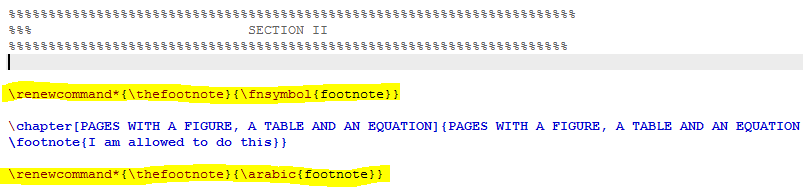
\includegraphics[scale=0.65]{Footnote.png}
	\caption{The inclusion of a copyright statement as a footnote. The lines in yellow help to change to footnote marking scheme.}
\end{figure}

\subsection{Another Test Section}
There should be things here.

%\begin{algorithm}
%Stuff.
%\end{algorithm}

\subsubsection{Test}
Hello, is it me you're looking for?

\subsubsection{Test 2}
There are more things to do.

\subsection{Yet Another One}
She called me late last night to say she loved me so.
 
 \subsection{No Surprises Here}
 Insert another song lyric here.
